\documentclass{article}
\usepackage[utf8]{inputenc}
\usepackage{hyperref}
\usepackage[letterpaper, portrait, margin=1in]{geometry}
\usepackage{enumitem}
\usepackage{amsmath}
\usepackage{booktabs}
\usepackage{graphicx}

\usepackage{titlesec}

\titleformat{\section}
{\normalfont\Large\bfseries}{\thesection}{1em}{}[{\titlerule[0.8pt]}]
  
\title{Homework 4 Answers}
\author{Economics 7103}
\date{ }
  
\begin{document}
  
\maketitle

\section{Python}

\begin{enumerate}
\item See figure \ref{fig:hw4_q1}.  Yes, there appear to be parallel trends in fish bycatch for the treatment and control group before January 2018.  It appears that the program caused an immediate and large decline in bycatch.
\begin{figure}[h]
    \centering
    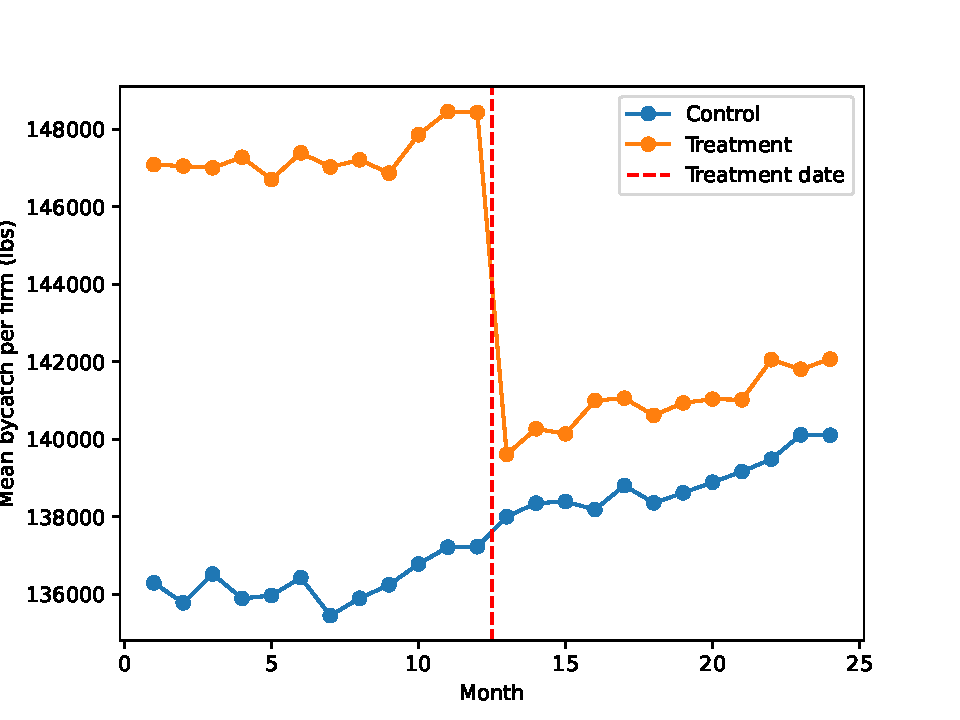
\includegraphics[scale = 0.7]{hw4_q1.pdf}
    \caption{Plot showing mean firm bycatch in pounds for months in 2017 and 2018.  Treatment occurred in January 2018.}
    \label{fig:hw4_q1}
\end{figure}
\item The estimate is -9,591, which implies that between December and January the average bycatch per firm in the treated group declined by 9,591 pounds relative to firms in the control group over the same period.
\item Output displayed in table on the next page.  The result is equivalent to the result in 2 (as we would expect).  As we add more rich controls, the estimated treatment effect declines, and the estimate becomes more precise.
\end{enumerate}

\begin{table}[!htbp] \centering
\begin{tabular}{@{\extracolsep{5pt}}lccc}
\\[-1.8ex]\hline
\hline \\[-1.8ex]
& \multicolumn{3}{c}{\textit{Dependent variable: bycatch}} \
\cr \cline{2-4}
\\[-1.8ex] & (1) & (2) & (3) \\
\hline \\[-1.8ex]
 Treated & -9591.35$^{}$ & -8956.78$^{}$ & -8436.28$^{***}$ \\
& (32619.42) & (9300.27) & (873.24) \\
 Treatment group & 11202.04$^{}$ & 11052.45$^{*}$ & -21.90$^{}$ \\
& (23065.41) & (6576.28) & (619.76) \\
 Pre-period & 773.22$^{}$ & & \\
& (23970.28) & & \\
 Shrimp & & & 1.06$^{***}$ \\
& & & (0.02) \\
 Salmon & & & 0.60$^{***}$ \\
& & & (0.07) \\
\hline \\[-1.8ex]
 Month indicators & Y & Y & Y \\
 Observations & 100 & 1200 & 1200 \\
 $R^2$ & 0.00 & 0.00 & 0.99 \\
 Adjusted $R^2$ & -0.03 & -0.02 & 0.99 \\
 Residual Std. Error & 81287.17 & 80284.53 & 7537.89 \\
 F Statistic & 0.10$^{}$ & 0.13$^{}$ & 4727.64$^{***}$ \\
\hline
\hline \\[-1.8ex]
\textit{Note:} & \multicolumn{3}{r}{$^{*}$p$<$0.1; $^{**}$p$<$0.05; $^{***}$p$<$0.01} \\
\end{tabular}
\end{table}



\clearpage

\section{Stata}
\begin{enumerate}
    \item  See table \ref{tab:hw4stata}.  Note the results from b are equivalent to a--the standard errors differ slightly.  There are issues with the standard errors for b in that the variance in the estimate of the firm mean values should be incorporated into the standard errors.  Most statistical packages take care of this automatically.
\end{enumerate}

\begin{table}[h]
    \centering
    \begin{tabular}{lcc} \hline
 & (1) & (2) \\
 & 1a & 1a \\
VARIABLES & 1b & 1b \\ \hline
 &  &  \\
Treated & -8,085*** &  \\
 & (2,619) &  \\
Shrimp & 1.552*** &  \\
 & (0.178) &  \\
Salmon & -0.680 &  \\
 & (1.125) &  \\
Treated - mean &  & -8,085*** \\
 &  & (2,564) \\
Shrimp - mean &  & 1.552*** \\
 &  & (0.175) \\
Salmon - mean &  & -0.680 \\
 &  & (1.101) \\
Constant & 199,615 & -861.8 \\
 & (245,802) & (1,161) \\
 &  &  \\
Observations & 1,200 & 1,200 \\
 R-squared & 0.996 & 0.428 \\ \hline
\multicolumn{3}{c}{ Robust standard errors in parentheses} \\
\multicolumn{3}{c}{ *** p$<$0.01, ** p$<$0.05, * p$<$0.1} \\
\end{tabular}

    \caption{Stata output}
    \label{tab:hw4stata}
\end{table}

\end{document}